\section{APPROACHES TO MULTIPLE OBJECT TRANSPORTATION}
\subsection{Transformable Multirotor with Two-dimensional Multilinks}
Zhao et al.\cite{Zhao2016} proposed a transformable multirotor comprising link modules with built-in propellers and achieved the stable aerial transformation. In another work\cite{ZhaoICRA2017}, they achieved the aerial manipulation by using the whole body of the transformable aerial robot. The joints with the same rotational axis allows the two-dimensional transformation as shown in \figref{multi_link}. In this work, we focus on the fact that this aerial robot has the ability to modify the position of CoG actively. Thus, this aerial robot can keep the flight stable by aerial transformation although the number of objects it grasps changes. Therefore, using this way, we approach to the multiple object transportation.
\begin{figure}[t]
  \begin{center}
    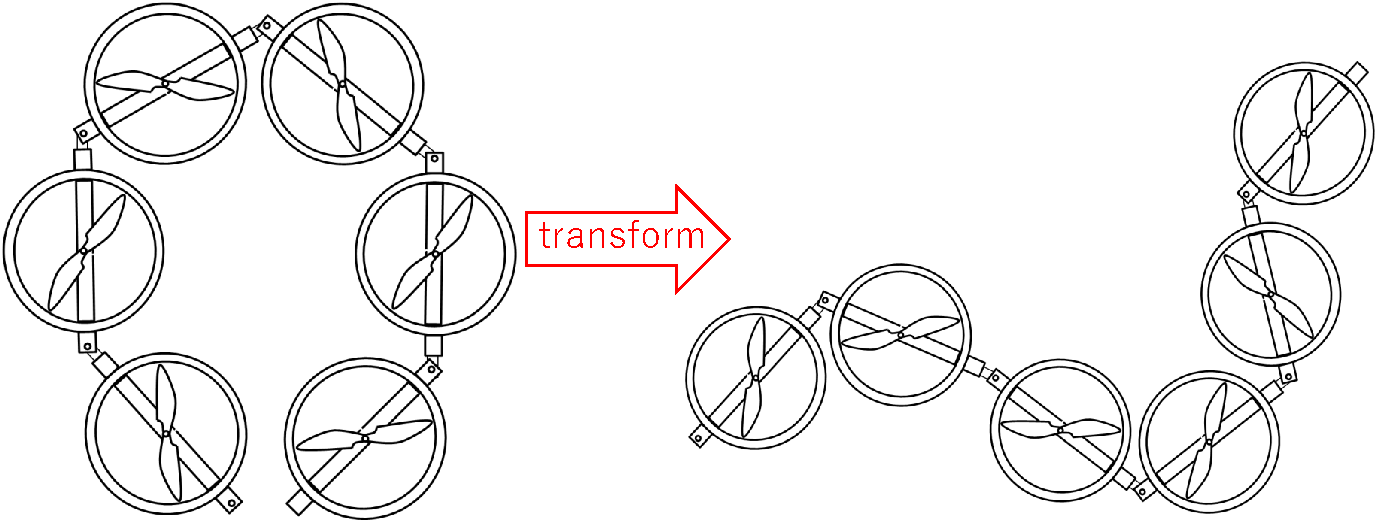
\includegraphics[width=1.0\columnwidth]{figs/multi_link.pdf}
  \end{center}
  \caption{multi link.\label{figure:multi_link}}
\end{figure}
 
\subsection{Form Optimization Based on Flight Stability}
To keep the flight stable by aerial transformation, the multirotor with multilinks must transform to a particular form. In this work, to obtain the form, we propose the method of form optimization based on flight stability. In Sec. IV, firstly, we investigate the definition of flight stability. Secondly, constraints of form considering the geometric condition and control stability is introduced. Finally, optimal form is obtained by using gradient descent.
  
\subsection{Hardware and Software System}
To transport objects by aerial robots, grippers are necessary for grasp objects. Hense, we develop an electromagnet gripper and whole hardware and software system including the link module of multilink and the multi-layer structure for internal communication. In Sec. V, we explain the system in detail.
